\documentclass{article}

% Language setting
% Replace `english' with e.g. `spanish' to change the document language
\usepackage[english]{babel}

% Set page size and margins
% Replace `letterpaper' with `a4paper' for UK/EU standard size
\usepackage[letterpaper,top=2cm,bottom=2cm,left=3cm,right=3cm,marginparwidth=1.75cm]{geometry}

% Useful packages
\usepackage{amsmath}
\usepackage{graphicx}
\usepackage{booktabs}
\usepackage{natbib}
\usepackage{float}
\usepackage[colorlinks=true, allcolors=blue]{hyperref}

\graphicspath{{figures/}}

\title{Image Colorization as Quantized Color Classification}
\author{Luke Dederich}
\date{December 4, 2026}

\begin{document}
\maketitle

\begin{abstract}
\noindent This project creates an encoder-decoder image colorization model from scratch with a U-Net style architecture. The goal of the model is to take a grayscale input (L) and produce a color output (ab). The model's output is quantized over ab color bins to produce vivid colors instead of the muddier results produced by models without this step. Muddiness is also mitigated through class rebalancing; rare, vivid colors are weighted more heavily than common colors. The model is trained on a subset of the Places365 dataset; only selected outdoor classes were used for this project. The model created in this project produces colorized results that typically look reasonable based on visual inspection. Furthermore, the model produced a 23.33 dB PSNR versus a 21.94 dB for the grayscale input. This is a notable result; beating the PSNR value of grayscale input means the model's color guesses are right more often than they are confidently wrong, resulting in plausible looking predictions. Colorfulness and visual inspection are used for evaluation in addition to PSNR/SSIM. Notably, a model without class rebalancing scores best on PSNR/SSIM (25.38 dB) but is duller than real photos (colorfulness 32.06 vs. 42.73). In the training process, random-crop augmentation gave the largest gain in these metrics.
\end{abstract}

\section{Introduction}

The goal of this project was to produce an encoder-decoder model that takes in a grayscale image as input and produces a plausible colorized image as output. The project works in the CIELab color space where the grayscale input images only have the lightness (L) channel and the predicted output provides the additional ‘a’ and ‘b’ color channels. This is a self-supervised learning task; the model does not require labeled data to train.

Image colorization technology has several uses. One use most people are familiar with is colorization for historical photos and films. Since historical media was captured before color camera technology, the media has no color information. Models such as the one created in this project can be used to predict plausible colors for the media and facilitate improved insights and entertainment from this imagery.

\subsection{Challenges}

\subsubsection{Plausible Colors for Gray Values}
Objects and surfaces can plausibly have several different colors, which presents a challenge for image colorization. For example, a field could be several different distinct colors, such as green, gold, or brown. A model trained on extensive data will have learned all of these colors, likely with no strong signal for a single color. As a result, models trained with regression loss tend to produce brownish or de-saturated results, ``averaging out'' the loss to prevent extensive penalties from confidently choosing an incorrect color~\citep{zhang2016colorful}.

\subsubsection{Class Imbalances}
Low saturation colors dominate the pixels, since they are more common. As a result, models trained without class rebalancing may not produce vivid colors \citep{zhang2016colorful}, even when they are an essential feature of the ground truth image. Figure~\ref{fig:ab_distribution} (left and middle panels) shows the distribution of training pixels across the color bins; note most pixels cluster in the middle.
 
\subsubsection{Evaluation}
Evaluating an image colorization model presents distinct challenges. Foremost is that there is no single correct answer; while outputs more similar to ground truth are considered better, the model can produce several outputs with different colors that vastly differ in quality upon visual inspection but differ little in similarity scores. Another challenge with evaluation traces back to the ``averaging out'' behavior described above. Peak signal-to-noise ratio (PSNR), the primary error calculation metric for image appearance differences, favors dull, cautious colors. As a result, dull and even grayscale images score deceptively high. Other metrics need to be examined in concert with PSNR to properly evaluate a model.

\subsection{Solution}
The above challenges are addressed in this project using the following mitigation techniques. To resolve tendencies for colorization models to produce dull colors, the model output is quantized into distinct ab color bins, and rare colors are weighted more heavily in the loss (class rebalancing). Grayscale-image filtering is used on the dataset prior to training to prevent the model from learning the ``color'' values of near black and white images. Additionally, annealed-mean decoding, skip connections, and random-crop augmentation are utilized to increase performance. Evaluation is completed using PSNR and SSIM combined with colorfulness values and visual inspection.

\subsection{Related Work}

This project draws from related works for colorization techniques. \citet{zhang2016colorful} is the primary basis for this project. It is a core image colorization paper, and it includes binning, class rebalancing, and an annealed mean. Additionally, the encoder-decoder network architecture follows U-Net~\citep{ronneberger2015unet}. \citet{iizuka2016color} take a different approach, running regression on ab values directly (no bins) and adding a scene-classification branch that supplies helpful context. This project instead treats colorization as classification, which avoids the desaturation problem that regression losses often create. \citet{larsson2016learning} also predict a distribution over color bins, similar to this project. However, they use a network pretrained on ImageNet rather than training from scratch.

\section{Method}

\subsection{Color Space and Preprocessing}
Training pairs can be automatically generated by converting each image to the CIELab color space, where the ‘L’ channel can be the input image and the ‘a’ and ‘b’ channels are the target. The L channel contains pixel values $[0, 100]$ that represent the lightness of each pixel. Taken alone, this channel is analogous to a black and white image. The a and b channels represent red to green and blue to yellow respectively, with natural colors falling within about $[-110, 110]$ (the grid range for Equation~\ref{eq:cell}) \citep{cie2004colorimetry}.

Images are resized to $64 \times 64$ (for swifter training) and converted to CIELab using the scikit-image library \citep{vanderwalt2014scikit}. After conversion, L is scaled to $[-1, 1]$ to help gradient descent converge \citep{lecun2012efficient} using the equation:

\begin{equation}
\tilde{L} = \frac{L}{50} - 1, \qquad L \in [0, 100]
\label{eq:lnorm}
\end{equation}

\subsection{Color Quantization}

\begin{figure}[htbp]
\centering
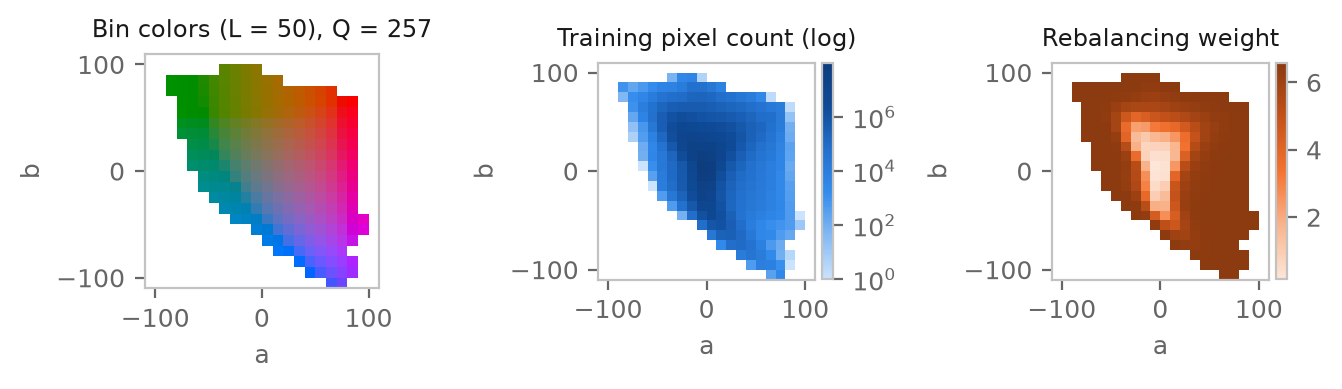
\includegraphics[width=\textwidth]{ab_distribution.png}
\caption{Bin Color and Pixel Count Distributions}
\label{fig:ab_distribution}
\end{figure}

Colors are quantized into bins to force the model to produce more vivid output. The indices are clamped to $[0, 21]$, which produces 484 cells:

\begin{equation}
i_a = \left\lfloor \frac{a + 110}{10} \right\rfloor, \qquad
i_b = \left\lfloor \frac{b + 110}{10} \right\rfloor, \qquad
k = 22\, i_a + i_b
\label{eq:cell}
\end{equation}

The cells that occur in the training data are calculated and kept as bins; all other cells are discarded. Each bin's color is its cell center, calculated as follows:

\begin{equation}
\mathbf{c}_q = \left(-110 + 10\, i_a + 5,\; -110 + 10\, i_b + 5\right)
\label{eq:centers}
\end{equation}

Figure~\ref{fig:ab_distribution} (left panel) shows the bin colors in ab values.

\subsection{Class Rebalancing}
Class rebalancing is used to avoid the model heavily favoring dull color bins. The below equation, utilized in this project for class rebalancing, is the work of~\citet{zhang2016colorful}.

\begin{equation}
w_q \propto \left( (1 - \lambda)\, p_q + \frac{\lambda}{Q} \right)^{-1},
\qquad \sum_{q=1}^{Q} p_q\, w_q = 1, \qquad \lambda = 0.5
\label{eq:weights}
\end{equation}

\noindent Note that $p_q$ is the fraction of training pixels in bin $q$. Unlike the paper~\citep{zhang2016colorful}, $p$ is not Gaussian-smoothed for simplicity. The resulting weights range from 0.17 to 6.57; see Figure~\ref{fig:ab_distribution} (middle and right panels).

\subsection{Network Architecture}

\begin{table}[htbp]
\centering
\small
\begin{tabular}{lp{0.42\textwidth}cc}
\toprule
Stage & Layers & Channels & Resolution \\
\midrule
Encoder 1 & $2\times$ (Conv $3\times3$, BN, ReLU), max-pool & $1 \rightarrow 32$ & $64 \rightarrow 32$ \\
Encoder 2 & $2\times$ (Conv $3\times3$, BN, ReLU), max-pool & $32 \rightarrow 64$ & $32 \rightarrow 16$ \\
Encoder 3 & $2\times$ (Conv $3\times3$, BN, ReLU), max-pool & $64 \rightarrow 128$ & $16 \rightarrow 8$ \\
Bottleneck & $2\times$ (Conv $3\times3$, BN, ReLU) & $128 \rightarrow 128$ & $8$ \\
Decoder 1 & Upsample $\times2$, concat Encoder 3, $2\times$ (Conv $3\times3$, BN, ReLU) & $128{+}128 \rightarrow 128$ & $16$ \\
Decoder 2 & Upsample $\times2$, concat Encoder 2, $2\times$ (Conv $3\times3$, BN, ReLU) & $128{+}64 \rightarrow 64$ & $32$ \\
Decoder 3 & Upsample $\times2$, concat Encoder 1, $2\times$ (Conv $3\times3$, BN, ReLU) & $64{+}32 \rightarrow 32$ & $64$ \\
Output & Conv $1\times1$, log-softmax & $32 \rightarrow Q = 257$ & $64$ \\
\midrule
\multicolumn{4}{l}{Total parameters: 1{,}219{,}521} \\
\bottomrule
\end{tabular}
\caption{Encoder-Decoder Architecture}
\label{tab:architecture}
\end{table}

\subsubsection{Layout}
An overview of the colorization network architecture is provided in Table~\ref{tab:architecture}. The most notable aspect of the architecture is the encoder-bottleneck-decoder layout. The encoder shrinks the image so that each bottleneck feature sees the entire scene, which is needed for the model to learn spatial information for similarly colored features, such as sky and water. The decoder restores full resolution for per-pixel predictions~\citep{long2015fully, ronneberger2015unet}. The output of the model is a probability distribution of bins at each pixel:

\begin{equation}
\hat{P}_{h,w}(q) = \frac{\exp\big(s_{h,w,q}\big)}{\sum_{q'=1}^{Q} \exp\big(s_{h,w,q'}\big)}
\label{eq:softmax}
\end{equation}

\noindent where $s_{h,w,q}$ is the output of the $1 \times 1$ convolution.


\subsubsection{Skip Connections}

\begin{figure}[htbp]
\centering
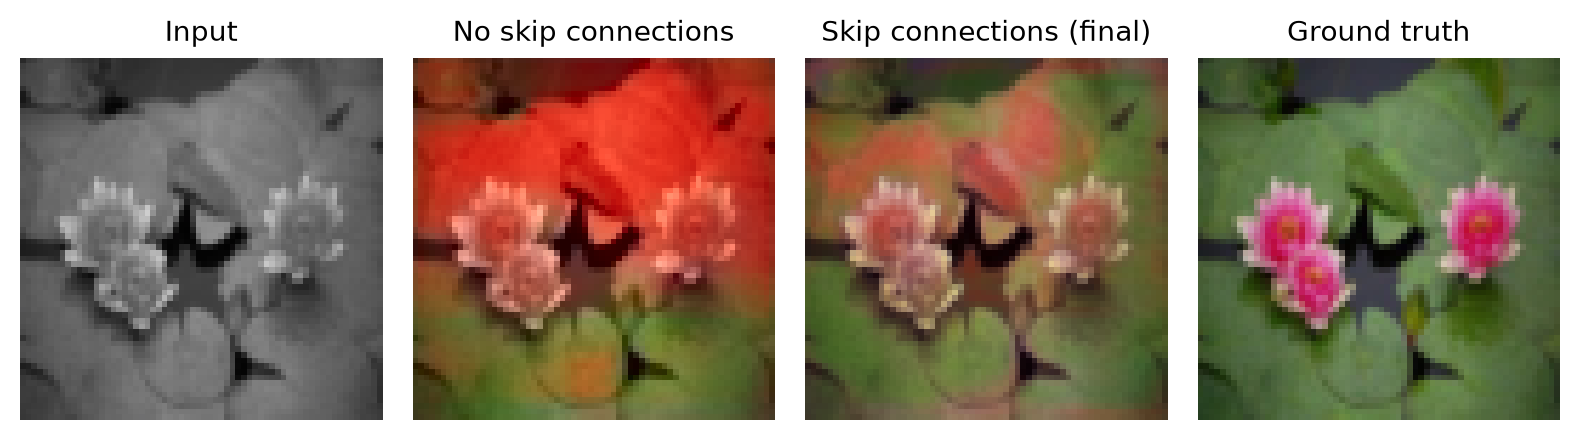
\includegraphics[width=\textwidth]{skip_compare.png}
\caption{Color Bleeding Without Skip Connections}
\label{fig:skip_compare}
\end{figure}

Skip connections are another aspect of the layout used for this project. Without them, color can spread across edges, such as in Figure~\ref{fig:skip_compare}. Since the bottleneck is only $8 \times 8$, without skip connections the decoder has to guess where the color edges are. Skip connections pass sharp encoder features to the decoder, which assists the decoder with aligning edges more properly~\citep{ronneberger2015unet}.

\subsubsection{Batch Normalization}
Batch normalization after each convolution stabilizes the training and allows for a higher learning rate \citep{ioffe2015batchnorm}.

\subsection{Loss}

This project uses PyTorch's \texttt{NLLLoss} function with custom class weights (from the class rebalancing described above) as the loss function. It divides by the sum of the weights, not the number of pixels.

\begin{equation}
\mathcal{L} = -\frac{\sum_{(h,w) \in \Omega} w_{z_{h,w}} \log \hat{P}_{h,w}\!\left(z_{h,w}\right)}
                   {\sum_{(h,w) \in \Omega} w_{z_{h,w}}}
\label{eq:loss}
\end{equation}

\noindent Note that $z_{h,w}$ is the true bin of pixel $(h, w)$ and $\Omega$ is the set of pixels whose cell is one of the kept bins (the rest are ignored).

\subsection{Decoding}

Decoding converts each pixel's predicted bin distribution into an ab color. The standard method, which was implemented initially for this project, uses argmax:

\begin{equation}
\hat{\mathbf{ab}}_{h,w} = \mathbf{c}_{q^*}, \qquad q^* = \arg\max_q \hat{P}_{h,w}(q)
\label{eq:argmax}
\end{equation}

\noindent However, to increase performance, the argmax decoding method was replaced with an annealed mean decoding method from~\citet{zhang2016colorful}:

\begin{equation}
f_T\big(\hat{P}\big)_q = \frac{\exp\big(\log \hat{P}(q) / T\big)}{\sum_{q'} \exp\big(\log \hat{P}(q') / T\big)},
\qquad
\hat{\mathbf{ab}}_{h,w} = \sum_{q=1}^{Q} f_T\big(\hat{P}_{h,w}\big)_q\, \mathbf{c}_q
\label{eq:annealed}
\end{equation}

\noindent \citet{zhang2016colorful} use $T=0.38$; for this project, the best visual results were produced by $T=0.7$, the value ultimately used.

\subsection{Training}

\begin{table}[htbp]
\centering
\begin{tabular}{ll}
\toprule
Setting & Value \\
\midrule
Input size & $64 \times 64$ \\
Training augmentation & Random resized crop (scale 0.4--1.0), horizontal flip \\
ab grid & $10 \times 10$ cells over $[-110, 110]$, $Q = 257$ bins used \\
Rebalancing $\lambda$ & 0.5 \\
Loss & Weighted cross-entropy (unused bins ignored) \\
Optimizer & SGD, momentum 0.9, weight decay $5 \times 10^{-4}$ \\
Learning rate & 0.01, cosine annealing \\
Batch size & 50 \\
Epochs & 60 (early stopping patience 8, best held-out loss kept) \\
Decoding & Annealed mean, $T = 0.7$ \\
Hardware & Apple GPU (MPS), $\approx 3.5$ min per epoch \\
\bottomrule
\end{tabular}
\caption{Training and Decoding Hyperparameters}
\label{tab:hyperparameters}
\end{table}

Training for this project was implemented in Python using the PyTorch library~\citep{paszke2019pytorch}. Table~\ref{tab:hyperparameters} shows the hyperparameters chosen for training. The optimizer settings follow \citet{krizhevsky2012imagenet}. Patience, the number of epochs, and temperature $T$ were then tuned experimentally. Early experimental runs used fewer epochs and a smaller set of data, allowing for swifter iteration than the final training configuration, which takes upwards of three hours per run on the available hardware.

Notable aspects of the training include random resized cropping of images~\citep{szegedy2015going}, early stopping on held-out loss, and a cosine learning-rate schedule~\citep{loshchilov2017sgdr}. Crops reduce overfitting (see Section 3.4.2) and early stopping keeps the checkpoint with the best held-out loss while cutting training short if loss is not improving after several epochs. Equation~\ref{eq:cosine} defines the learning rate decay, where $e$ represents the current epoch and $E$ represents the total epochs.

\begin{equation}
\eta_e = \frac{\eta_0}{2}\left(1 + \cos\!\left(\frac{\pi e}{E}\right)\right),
\qquad \eta_0 = 0.01
\label{eq:cosine}
\end{equation}

\section{Experiments}

\subsection{Dataset}
This project uses the Places365 standard dataset (\texttt{torchvision.datasets.Places365} \citep{zhou2018places}). This dataset was chosen because the Places dataset has been used in multiple colorization research papers \citep[e.g.,][]{iizuka2016color}, indicating it is a reasonable choice for this task. Furthermore, as a dataset available through \texttt{torchvision}, Places365 also allowed for smooth integration with the rest of this project, which uses PyTorch extensively. Additionally, the images provide more interesting environments for colorization as opposed to other common image datasets such as ImageNet. Only a subset of Places365 was used. The full dataset is about 1.8 million images, which is prohibitively large; using all of the images would not be feasible on the available hardware and timeline. Images are also downsized to $64 \times 64$ for more efficient training.

\subsubsection{Class Selection}
Exclusively outdoor scene categories were selected; these scenes have strong colors, which suits the model well. Outdoor spaces typically have more predictable colors (for example, foliage is typically green) unlike indoor spaces where the majority of objects could reasonably be several different colors. Twenty outdoor classes were initially selected, grouped by dominant color (Table~\ref{tab:classes}). Twenty additional classes were added for training only; all evaluation uses the initial twenty classes.

\begin{table}[htbp]
\centering
\small
\begin{tabular}{lp{0.68\textwidth}}
\toprule
Group & Places365 classes \\
\midrule
Water / coast & beach, coast, ocean, lagoon, lake/natural, waterfall \\
Vegetation & forest/broadleaf, rainforest, bamboo\_forest, field/wild, pasture, rice\_paddy, botanical\_garden \\
Fields / sand & wheat\_field, hayfield, desert/sand \\
Rock / terrain & canyon, badlands, butte, valley \\
\midrule
Extra (training only) & mountain, mountain\_snowy, cliff, creek, river, islet, swamp, marsh, pond, orchard, vineyard, corn\_field, field/cultivated, forest\_path, forest\_road, tree\_farm, desert/vegetation, rock\_arch, lawn, field\_road \\
\bottomrule
\end{tabular}
\caption{Places365 Classes Used}
\label{tab:classes}
\end{table}

\subsubsection{Dataset Splits}

\begin{table}[htbp]
\centering
\begin{tabular}{llcrrr}
\toprule
Split & Source & Classes & Before filtering & Train & Held-out / Test \\
\midrule
Train (target classes) & train-standard & 20 & 100{,}000 & 78{,}091 & 19{,}514 \\
Train (final model) & train-standard & 40 & 200{,}000 & 155{,}858 & 38{,}944 \\
Test & val & 20 & 2{,}000 & -- & 1{,}955 \\
\bottomrule
\end{tabular}
\caption{Image Counts Per Split, Before and After Grayscale Filtering}
\label{tab:splits}
\end{table}

The data was split 80/20 between training and held-out within each class (Table~\ref{tab:splits}). This method ensures that the training and held-out splits both have sufficient representation of every class. A hard-coded seed is used for splitting to produce identical splits each time the model is trained. The official Places365 val split is the test set, and is never used for training or tuning.

\subsubsection{Grayscale Filtering}
Grayscale filtering is implemented on the dataset to prevent the model from learning the color values of near black and white photos. Since the goal of the model is colorization, learning grayscale images, even if correct, would deviate from the goal. Grayscale filtering is performed using the chroma value of each image as shown in Figure~\ref{fig:chroma_bands}.

\begin{figure}[htbp]
\centering
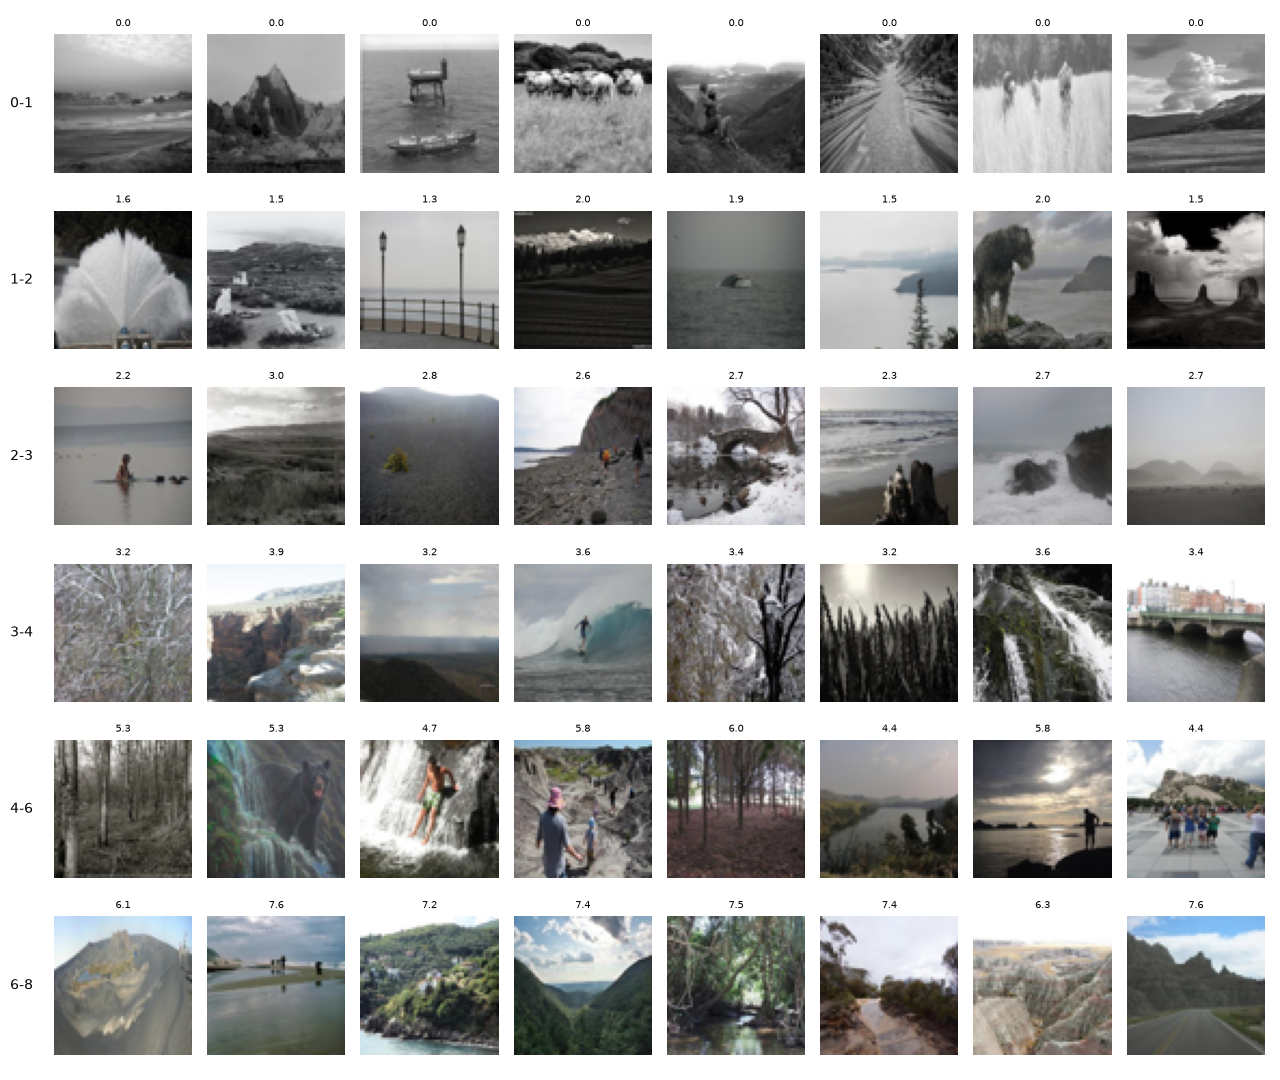
\includegraphics[width=\textwidth]{chroma_bands.png}
\caption{Random Training Images Grouped by Mean Chroma}
\label{fig:chroma_bands}
\end{figure}

Note that upon physical inspection images with a chroma value below 2 largely appear black and white, whereas images with chroma values between 2 and 3 start to introduce dull colors. For this reason, images with $\bar{C} < 2$ were removed from the dataset: 5,198 training images and 45 test images. Chroma ($\bar{C}$) values were calculated using Equation~\ref{eq:chroma} \citep{cie2004colorimetry}:

\begin{equation}
\bar{C} = \frac{1}{HW} \sum_{h,w} \sqrt{a_{h,w}^2 + b_{h,w}^2}
\label{eq:chroma}
\end{equation}

\subsection{Evaluation Metrics}
The model was evaluated using the below metrics along with visual inspection. These metrics were combined to overcome the grayscale-favoring issue posed in the introduction. All metrics are computed per image on RGB values in $[0, 1]$ and averaged over the 1,955 test images. Evaluation results are given in Table~\ref{tab:final_results}.

\subsubsection{Peak Signal-to-Noise Ratio (PSNR)}
Peak signal-to-noise ratio, or PSNR, is a metric that calculates the ratio of the maximum possible pixel value to the mean squared error (MSE) on a log scale; higher is better~\citep{huynh2008scope}. It was used in this project because it is the standard pixel-wise fidelity metric, used in landmark colorization works such as \citet{larsson2016learning}.

\begin{equation}
\mathrm{MSE} = \frac{1}{3HW} \sum_{h,w,c} \big(\hat{I}_{h,w,c} - I_{h,w,c}\big)^2,
\qquad
\mathrm{PSNR} = 10 \log_{10}\!\left(\frac{1}{\mathrm{MSE}}\right)
\label{eq:psnr}
\end{equation}

where $I$ and $\hat{I}$ are the ground-truth and predicted RGB images, $H \times W$ is the image size, and $c$ indexes the three color channels. The numerator is 1 because pixel values lie in $[0, 1]$.

\subsubsection{Structural Similarity (SSIM)}
Structural Similarity, or SSIM, is a metric that compares local mean, variance, and covariance between windows, with a maximum of 1~\citep{wang2004ssim}. It was used in this project because it captures structure that per-pixel error misses.

\begin{equation}
\mathrm{SSIM}(x, y) = \frac{(2\mu_x \mu_y + C_1)(2\sigma_{xy} + C_2)}
                           {(\mu_x^2 + \mu_y^2 + C_1)(\sigma_x^2 + \sigma_y^2 + C_2)}
\label{eq:ssim}
\end{equation}

where $x$ and $y$ are corresponding windows of the two images, $\mu$ and $\sigma^2$ are the window means and variances, $\sigma_{xy}$ is their covariance, and $C_1$, $C_2$ are small constants that prevent division by zero. The project used $7 \times 7$ windows, averaged over windows and RGB channels, with $C_1 = 0.01^2$ and $C_2 = 0.03^2$.

\subsubsection{Colorfulness}
Colorfulness is a metric that measures how colorful an image is. This is an important measurement to use in concert with the previous ones because unlike PSNR/SSIM, which favor dull outputs, colorfulness does not. Colorfulness has no ``better'' direction; colorfulness values are compared between a prediction and ground truth, with smaller differences being better. The colorfulness equation used for this project was created by~\citet{hasler2003colorfulness}.

\begin{equation}
rg = R - G, \qquad yb = \tfrac{1}{2}(R + G) - B
\end{equation}
\begin{equation}
M = \sqrt{\sigma_{rg}^2 + \sigma_{yb}^2} + 0.3\sqrt{\mu_{rg}^2 + \mu_{yb}^2}
\label{eq:colorfulness}
\end{equation}

where $R$, $G$, $B$ are channel values in $[0, 255]$, and $\sigma$ and $\mu$ are the standard deviation and mean of the opponent channels $rg$ and $yb$ over all pixels. The first term measures how varied the colors are and the second measures the overall color cast.

\subsection{Results}

This project produced a model that colorizes grayscale images plausibly with generally visually appealing results. The primary quantitative results of the best model are given in Table~\ref{tab:final_results}. The PSNR of the model is 23.33 dB vs. 21.94 dB for the baseline gray input (+1.39 dB, about $27\%$ lower squared error). This result is notable because it means despite the ``averaging out'' problem described at the beginning of this paper, the model outperformed the gray baseline. This means the model chose correct colors more often than being confidently wrong, while also producing results with color details.

The SSIM for the baseline and the colorized predictions are very similar (0.9003 vs. 0.8992). This can be considered a tie because the difference is about $0.1\%$, a negligible difference. Note that increasing the annealed mean $T$ value results in a higher SSIM value, but this ends up sacrificing a visually unsatisfying amount of vividness.

Colorfulness is the main check against dull output. The model scored 48.59 as opposed to 42.73 for ground truth, which means it is more vivid than the ground truth. $T = 0.7$ slightly over-saturates (see Section 3.4.3). As expected, the gray baseline input has a colorfulness value of 0.

\begin{table}[htbp]
\centering
\begin{tabular}{lccc}
\toprule
Output & PSNR (dB) $\uparrow$ & SSIM $\uparrow$ & Colorfulness \\
\midrule
Gray input ($ab = 0$) & 21.94 & 0.9003 & 0.00 \\
Argmax & 21.77 & 0.8322 & 57.38 \\
Annealed mean, $T = 0.38$ & 22.89 & 0.8891 & 51.67 \\
Annealed mean, $T = 0.5$ & 23.08 & 0.8938 & 50.48 \\
\textbf{Annealed mean, $T = 0.7$} & \textbf{23.33} & \textbf{0.8992} & \textbf{48.59} \\
Annealed mean, $T = 1.0$ & 23.62 & 0.9043 & 45.62 \\
\midrule
Ground truth & -- & -- & 42.73 \\
\bottomrule
\end{tabular}
\caption{Final Model on the Filtered Test Set}
\label{tab:final_results}
\end{table}

Figure~\ref{fig:qualitative} shows some example results of the model, which are evenly spaced throughout the test set, not hand-selected. In all of the examples, the model produces a plausible result. In some cases, such as the example in the bottom right, it produces a more saturated result. The model does particularly well with skies and vegetation. In cases where there are small vivid portions of a photo, it sometimes fails to properly colorize them. One example is the photo of a bird in the grass in the top right. While the bird and its surroundings are not green in the truth, the model predicts color similar to the surrounding grass.

\begin{figure}[htbp]
\centering
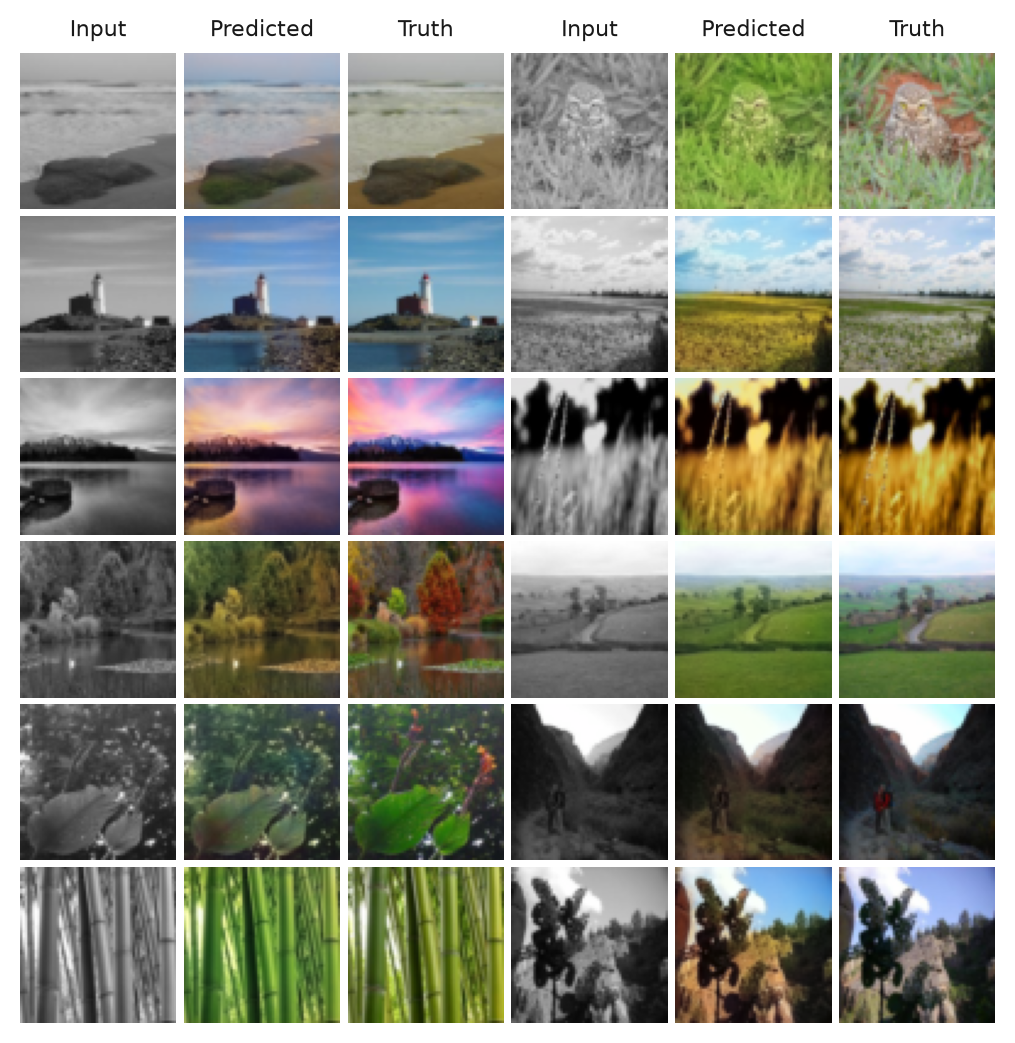
\includegraphics[width=0.9\textwidth]{qualitative.png}
\caption{12 Test Images: Input, Prediction, Ground Truth}
\label{fig:qualitative}
\end{figure}

\subsection{Analysis and Discussion}
\subsubsection{Architecture and Training Changes}
The architecture and training of the model went through several iterations before the final configuration was selected. These changes are enumerated in Table~\ref{tab:ablation}.

\begin{table}[htbp]
\centering
\begin{tabular}{lccccc}
\toprule
Model & Classes & Epochs (best) & PSNR (dB) $\uparrow$ & SSIM $\uparrow$ & Colorfulness \\
\midrule
Gray input & -- & -- & 21.94 & 0.9003 & 0.00 \\
\midrule
U-Net, no crop & 20 & 40 (27) & 22.88 & 0.8929 & 48.49 \\
+ random crop & 20 & 40 (40) & 23.17 & 0.8985 & 48.20 \\
+ 20 more epochs & 20 & 60 (58) & 23.24 & 0.8988 & 48.35 \\
+ extra training classes (final) & 40 & 60 (60) & 23.33 & 0.8992 & 48.59 \\
\midrule
Final, no skip connections & 40 & 60 (60) & 23.38 & 0.9022 & 47.32 \\
Final, no class rebalancing & 40 & 60 (60) & 25.38 & 0.9224 & 32.06 \\
\midrule
Ground truth & -- & -- & -- & -- & 42.73 \\
\bottomrule
\end{tabular}
\caption{Contribution of Each Change on the Filtered Test Set ($T = 0.7$)}
\label{tab:ablation}
\end{table}

Random cropping produced the largest gain of PSNR with +0.29 dB. Adding 20 extra epochs yielded a gain of +0.07 dB. Finally, adding extra data gave a +0.09 dB improvement, at the expense of significantly longer training time. 

Note the bottom two rows of the table. One run was performed using no class rebalancing. It has the best PSNR and SSIM of any model, but it yields a colorfulness well below the ground truth value. This reinforces the evidence that PSNR/SSIM reward dull output, and class rebalancing is needed to make the colors vivid. The model without skip connections has fewer parameters, and has a worse held-out loss. The metrics are similar to the final model, but there is a notable visible trade-off: without skips the color sometimes bleeds across boundaries; with skips, the color follows better along edges.

\subsubsection{Overfitting}
Without random cropping, held-out loss bottoms out at epoch 27 while the train loss keeps falling, indicating overfitting. As shown in Figure~\ref{fig:loss_curves}, with cropping held-out loss improves through to the last epoch, epoch 40.

\begin{figure}[htbp]
\centering
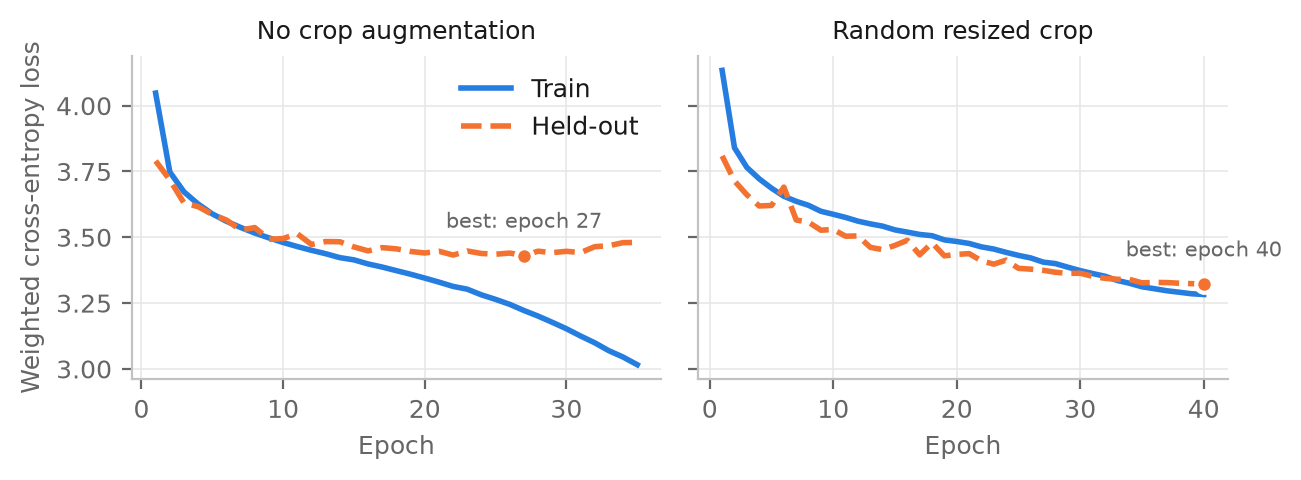
\includegraphics[width=\textwidth]{loss_curves.png}
\caption{Effect of Cropping on Weighted Cross-Entropy Loss}
\label{fig:loss_curves}
\end{figure}

In early experimentation, a larger model with 64 channels overfit even more, with held-out loss improvement stopping at even earlier epochs.

\subsubsection{Decoding Temperature}
Recall that decoding converts each pixel's predicted bin distribution into an ab color. Two methods of decoding were tested in this project: argmax and annealed mean. Argmax is the most vivid but evaluates the worst on PSNR/SSIM. For this reason, annealed mean decoding~\citep{zhang2016colorful} was used instead. Annealed mean decoding takes in an important hyperparameter, temperature ($T$). Several values were tried in this project. Raising $T$ improves PSNR/SSIM while colorfulness falls (Figure~\ref{fig:temperature}). The metrics reward desaturation, and $T = 0.7$ is a compromise to ensure vivid colors, one of the goals of this project. Image vividness variation from $T$ is shown in Figure~\ref{fig:decoding}.

\begin{figure}[htbp]
\centering
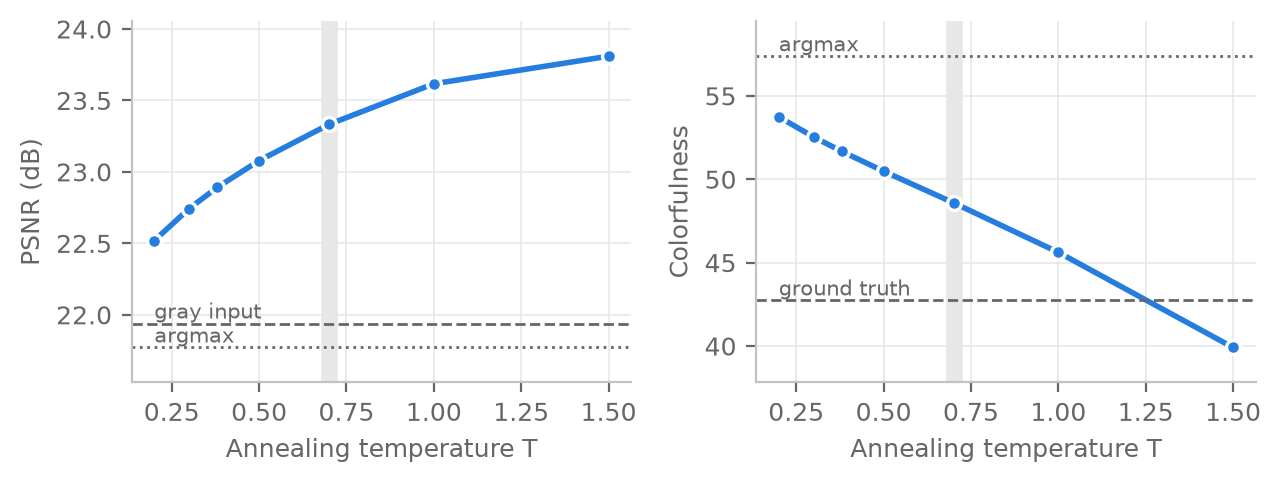
\includegraphics[width=0.9\textwidth]{temperature.png}  
\caption{Effect of Temperature on PSNR and Colorfulness}
\label{fig:temperature}
\end{figure}

\begin{figure}[H]
\centering
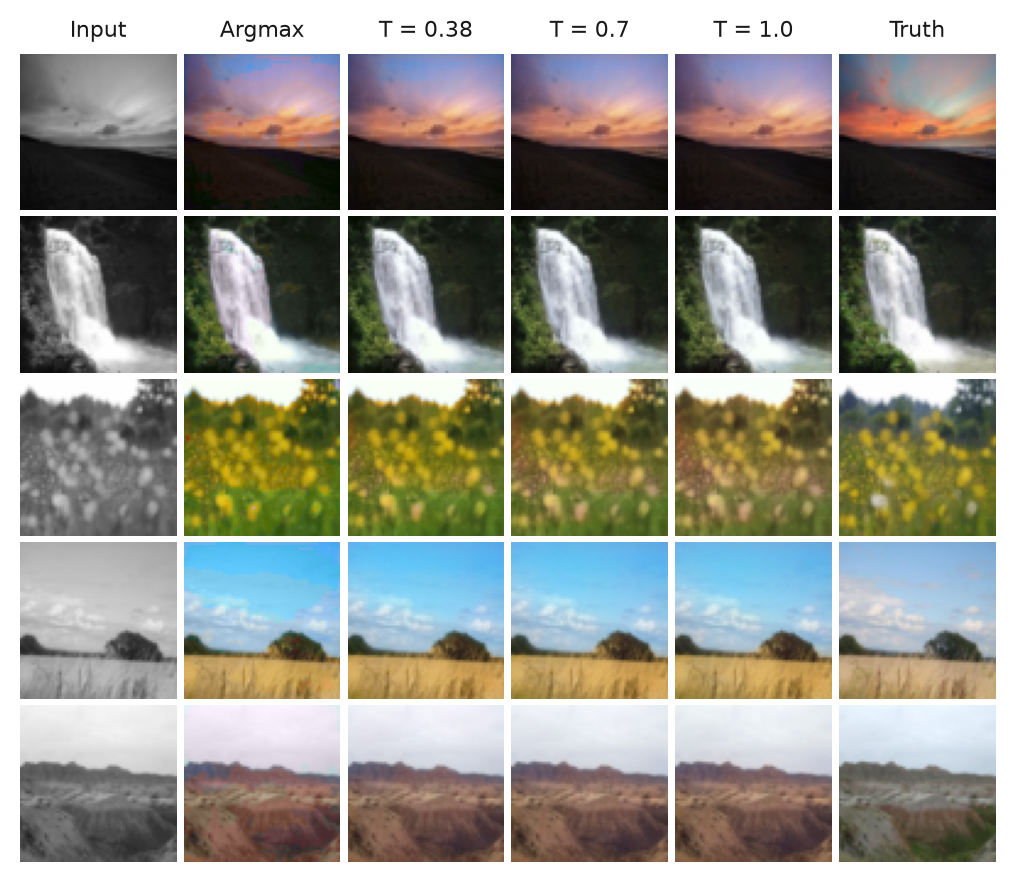
\includegraphics[width=0.8\textwidth]{decoding.png} 
\caption{Effect of Varied Decoding on Model Predictions}
\label{fig:decoding}
\end{figure}

\subsubsection{Grayscale Filtering}

\begin{table}[H]
\centering
\begin{tabular}{lrcccc}
\toprule
 & & \multicolumn{2}{c}{Gray input} & \multicolumn{2}{c}{Final model ($T = 0.7$)} \\
\cmidrule(lr){3-4} \cmidrule(lr){5-6}
Test set & Images & PSNR (dB) & SSIM & PSNR (dB) & SSIM \\
\midrule
Unfiltered val & 2{,}000 & 23.41 & 0.9025 & 23.27 & 0.8988 \\
Filtered val (chroma $\geq 2$) & 1{,}955 & 21.94 & 0.9003 & 23.33 & 0.8992 \\
\bottomrule
\end{tabular}
\caption{Effect of Grayscale Filtering}
\label{tab:filtering}
\end{table}

Table~\ref{tab:filtering} shows the effect of grayscale filtering on model PSNR/SSIM performance. The same model loses to gray on the unfiltered test set (23.27 versus 23.41) but wins over gray on the filtered set. This behavior is because for nearly grayscale images, the true ab is close to 0, so the gray baseline is nearly correct.

\subsubsection{Skip Connections}

As discussed previously, skip connections did not notably improve the metrics, but they improved color localization and reduced bleeding in some images (Figure~\ref{fig:skip_compare}), at the cost of patchier local errors in others.

\subsubsection{Amount of Training Data}
\begin{figure}[htbp]
\centering
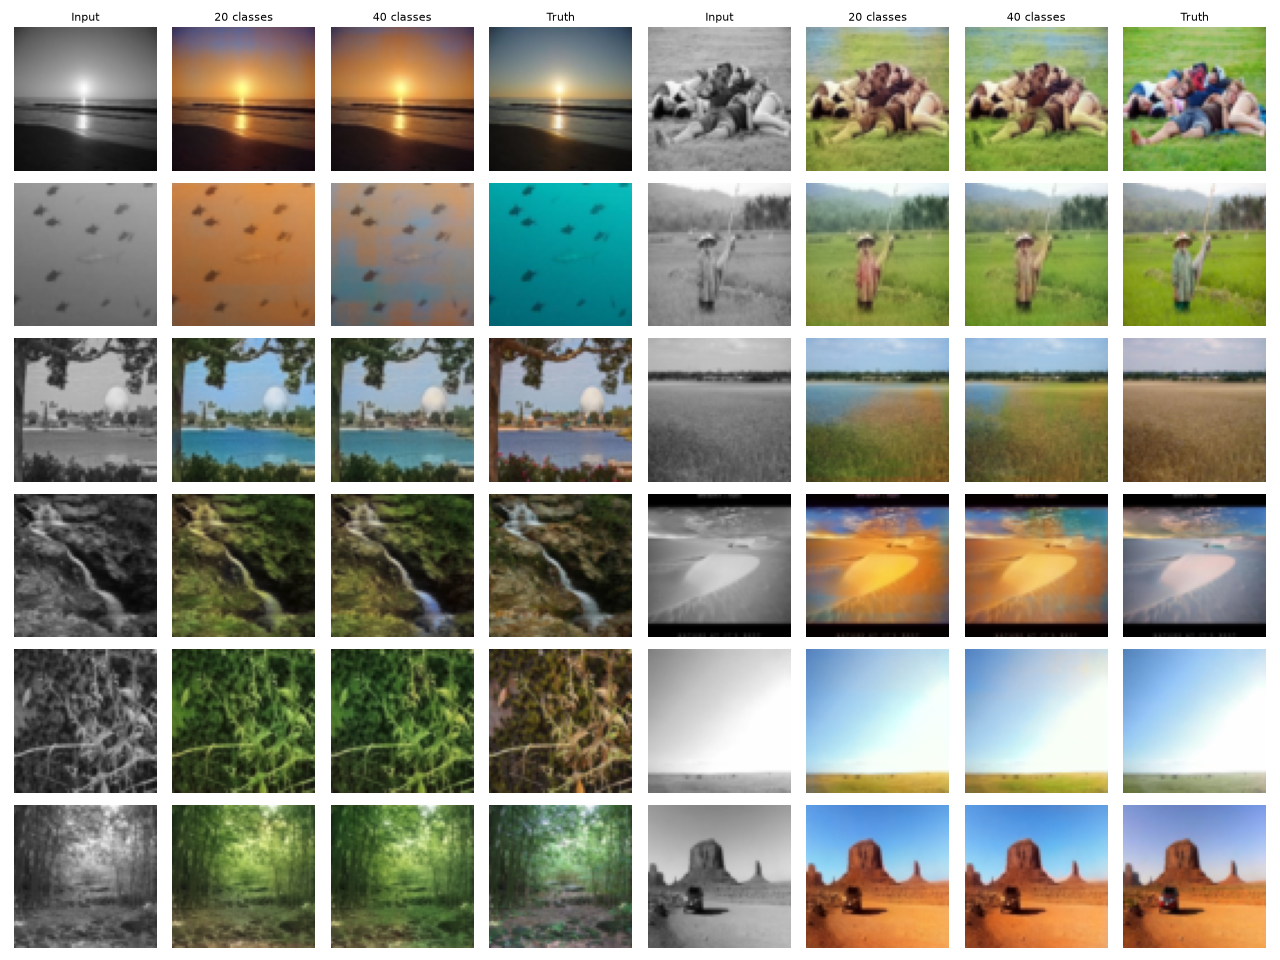
\includegraphics[width=0.9\textwidth]{data_compare.png}
\caption{Model Trained on 20 Classes vs. 40 Classes}
\label{fig:data_compare}
\end{figure}

The models were additionally trained on 20 classes; 20 additional classes were added later (for a total of 40 classes) to improve model performance. This yielded only small metric gains and took significantly longer, but produced visible fixes. One notable example in Figure~\ref{fig:data_compare} is the waterfall photo, which gains a ``water blue'' color in the 40 class model that was not present in the 20 class model.

\subsubsection{Failure Cases}
While the model generally produces results near the truth, it is not perfect. Figure~\ref{fig:failures} shows selected failure cases of the model, where it produces results that look significantly different than the ground truth. These are rare cases among outdoor scenes that are highly ambiguous in color when examining only the grayscale images. In some of these cases, the model produces results that could theoretically be correct learned from other images. An example of this is the photo in the bottom right of Figure~\ref{fig:failures}. Here, the model produced colors consistent with a sunset sky, rather than a daytime one. This behavior extends to the worse examples in the top row, where the model is likely treating the water as sky and applying some of the same orange sunset-like colors.

\begin{figure}[htbp]
\centering
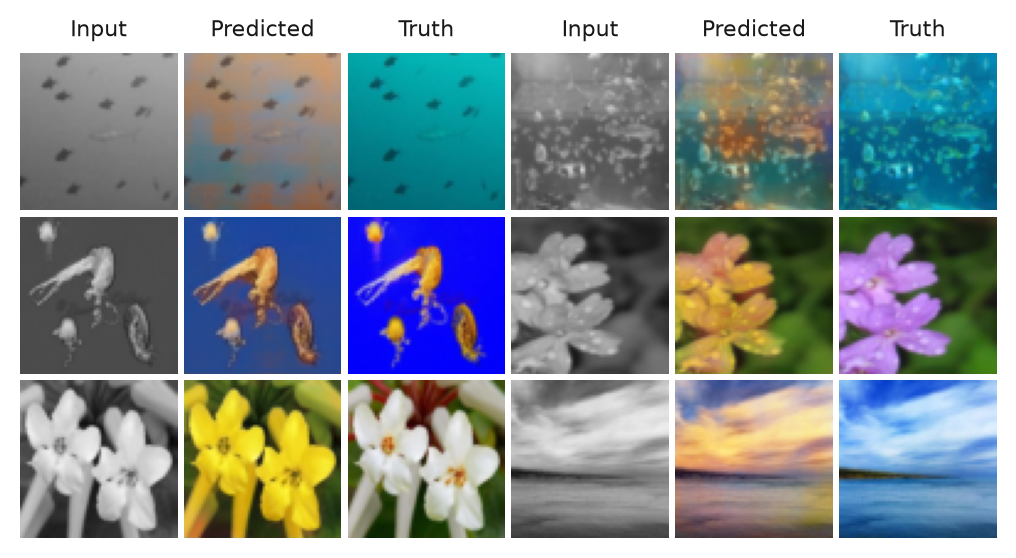
\includegraphics[width=0.9\textwidth]{failures.png}
\caption{6 Test Images with the Lowest PSNR Values}
\label{fig:failures}
\end{figure}

\subsubsection{Limitations}
This project has some limitations worth noting here. First of all, generally only one training run was done per configuration. This means that metric variance between runs of identical configurations was not considered. Furthermore, this project was run on images downsized to $64 \times 64$. These are very small images, and real-world tasks would likely need a model that runs on larger images.

\section{Conclusion}
This project produced an encoder-decoder image colorization model that generally produces plausible results. One of the most notable learnings from this project is the gap between what the metrics reward and what actually produces reasonable colorized images. Implementing colorfulness to mitigate the grayscale favoring from PSNR/SSIM metrics was an essential step that was not expected going into this project. Furthermore, the effect of data cleaning and preprocessing was unexpected. The gains produced just from introducing random cropping and grayscale filtering were remarkable.

There is still room to improve this model. A scene-classification head \citep{iizuka2016color}, a higher resolution, a larger model, and a human perceptual study could all expand upon this project and produce a better model.

\newpage
\bibliographystyle{plainnat}
\bibliography{references}

\end{document}